%%%%%%%%%%%%%%%%%%%%%%%%%%%%%%%%%%%%%%%%%
% Short Sectioned Assignment
% LaTeX Template
% Version 1.0 (5/5/12)
%
% This template has been downloaded from:
% http://www.LaTeXTemplates.com
%
% Original author:
% Frits Wenneker (http://www.howtotex.com)
%
% License:
% CC BY-NC-SA 3.0 (http://creativecommons.org/licenses/by-nc-sa/3.0/)
%
%%%%%%%%%%%%%%%%%%%%%%%%%%%%%%%%%%%%%%%%%

%-------------------------------------------------------------------------------
%	PACKAGES AND OTHER DOCUMENT CONFIGURATIONS
%-------------------------------------------------------------------------------

\documentclass[paper=a4, fontsize=11pt]{scrartcl} % A4 paper and 11pt font size
\usepackage{geometry} % Pour passer au format A4
\geometry{hmargin=1cm, vmargin=1cm} % 

\usepackage[T1]{fontenc} % Use 8-bit encoding that has 256 glyphs
\usepackage[english,francais]{babel} % Français et anglais
\usepackage[utf8]{inputenc} 

\usepackage{amsmath,amsfonts,amsthm} % Math packages

\usepackage{enumitem}
\usepackage{lmodern}
\usepackage{url}
\usepackage{eurosym} % signe Euros
\usepackage{geometry} % Pour passer au format A4
\usepackage{graphicx} % Required for including pictures
\usepackage{float} % Allows putting an [H] in \begin{figure} to specify the exact location of the figure

\usepackage{multicol}

\usepackage{verbatim}

\usepackage{sectsty} % Allows customizing section commands
\allsectionsfont{\centering \normalfont\scshape} % Make all sections centered, the default font and small caps

%------------------------------------------------------------------------------
%	Pied de Page
%------------------------------------------------------------------------------

\usepackage{fancyhdr} % Custom headers and footers
\pagestyle{fancyplain} % Makes all pages in the document conform to the custom headers and footers
\fancyhead{} % No page header - if you want one, create it in the same way as the footers below
\fancyfoot[C]{Cosinus dans un triangle rectangle} % Empty center footer
\fancyfoot[R]{\thepage} % Page numbering for right footer

\renewcommand{\headrulewidth}{0pt} % Remove header underlines
\renewcommand{\footrulewidth}{0pt} % Remove footer underlines


\setlength\parindent{0pt} % Removes all indentation from paragraphs - comment this line for an assignment with lots of text


%------------------------------------------------------------------------------
%	Titre
%-----------------------------------------------------------------------------

\newcommand{\horrule}[1]{\rule{\linewidth}{#1}} % Create horizontal rule command with 1 argument of height


\title{	
  \vspace{-7ex}
  \horrule{0.5pt} \\[0.4cm] % Thin top horizontal rule
  \huge Cosinus d'un angle dans un triangle rectangle
  \horrule{2pt} \\[0.5cm] % Thick bottom horizontal rule
}

\author{}
\date{\vspace{-10ex}} % Today's date or a custom date

%--------------------------------------------------------------------------------
%	Début du document
%--------------------------------------------------------------------------------

\begin{document}

%-------------------------------------------------------------------------------
% RE-DEFINITION
%-------------------------------------------------------------------------------
% MATHS
%-----------

\newtheorem{Definition}{Définition}
\newtheorem{Theorem}{Théorème}
\newtheorem{Proposition}{Propriété}

% MATHS
%-----------
\renewcommand{\labelitemi}{$\bullet$}
\renewcommand{\labelitemii}{$\circ$}
%-------------------------------------------------------------------------------
%	Titre
%-------------------------------------------------------------------------------

\maketitle % Print the title
\setlength{\columnseprule}{1pt}

\subsection*{I - Formule}

\begin{multicols}{2}
  \begin{Definition}
    Dans un triangle \textbf{rectangle}.\\
    $$\text{cosinus d'un angle} = \dfrac{\text{longueur de l'adjacent à l'angle}}{\text{longueur de l'hypoténuse}}$$ 
  \end{Definition}

  \begin{Definition}
    EFG,  un triangle \textbf{rectangle} en E.\\
    $$\cos(\overbrace{EFG}) = \dfrac{FE}{FG}$$

  \end{Definition}

  \begin{figure}[H]
	  \centering
	  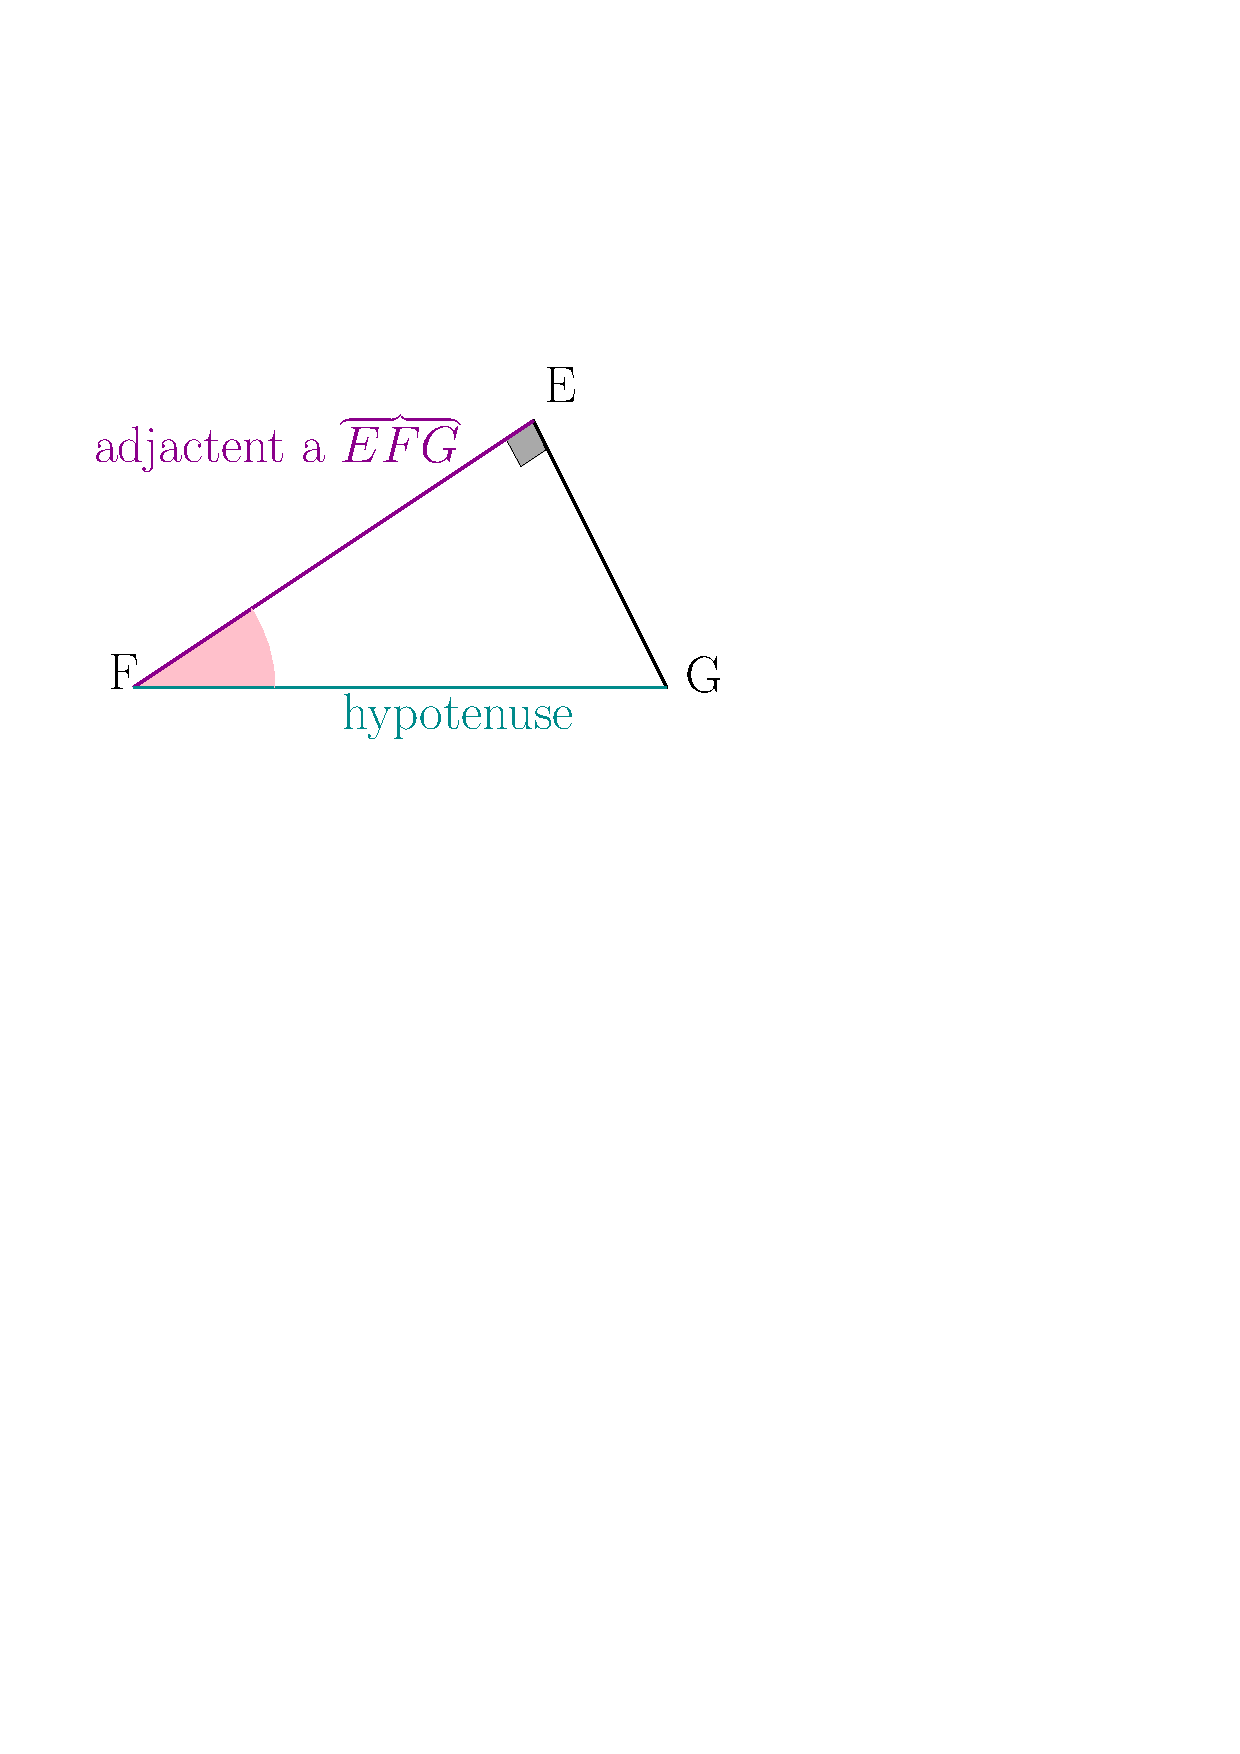
\includegraphics[width=0.8\linewidth]{sources/2/tri-EFG.pdf}
  \end{figure}

\end{multicols}

\paragraph{Remarques}~~\\
\begin{itemize}
\item La lettre au centre de l'angle se répète deux fois dans la formule du cosinus.
\item Le cosinus d'un angle dans un triangle rectangle est toujours compris entre 0 et 1.
\end{itemize}

 \horrule{0.5pt}
\subsection*{II - Trouver une longueur ou une mesure manquante dans un triangle rectangle}

\begin{multicols}{3}
  
  \subsubsection*{a) Recherche de l'adjacent}
  \begin{figure}[H]
	  \centering
	  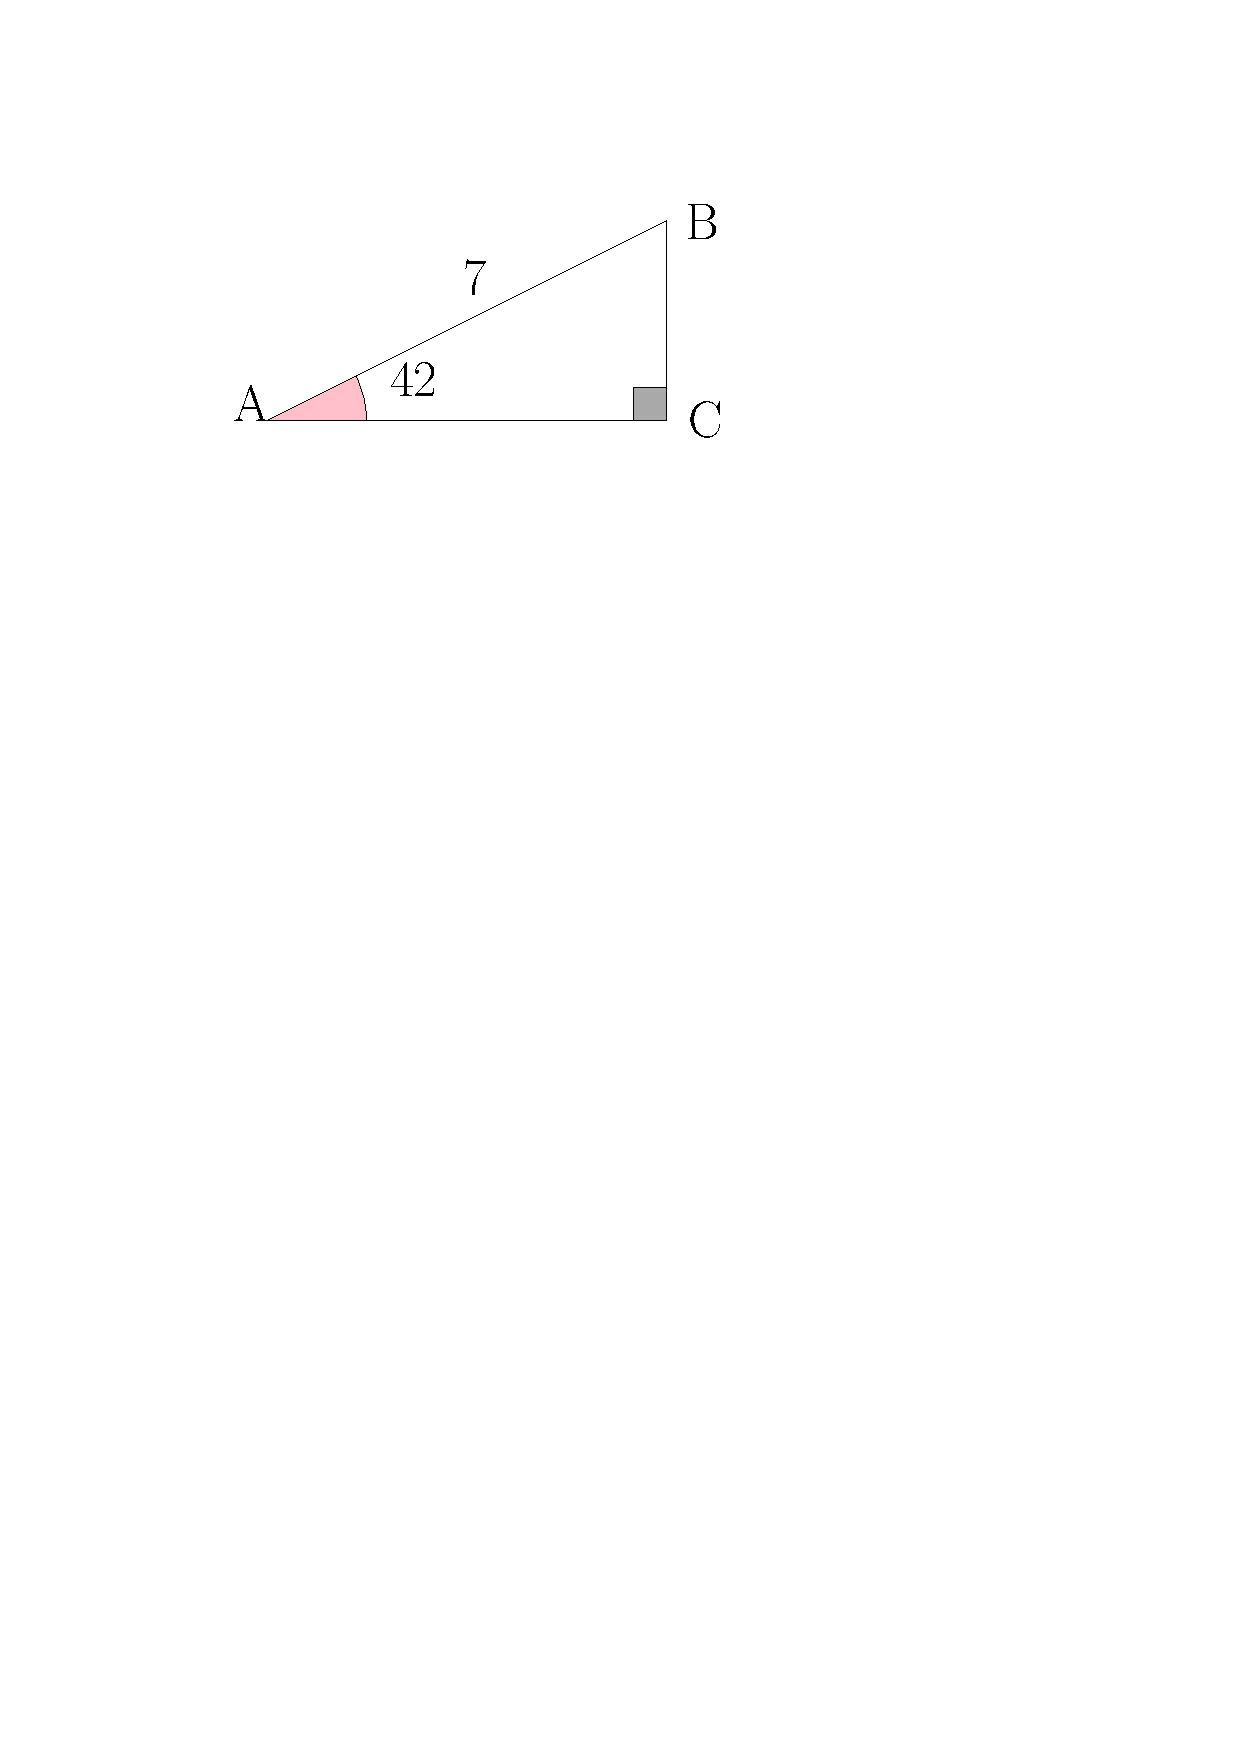
\includegraphics[width=0.8\linewidth]{sources/2/rec-a1.pdf}
	\end{figure}

  \subsubsection*{b) Recherche de l'hypoténuse}
  
  \begin{figure}[H]
	  \centering
	  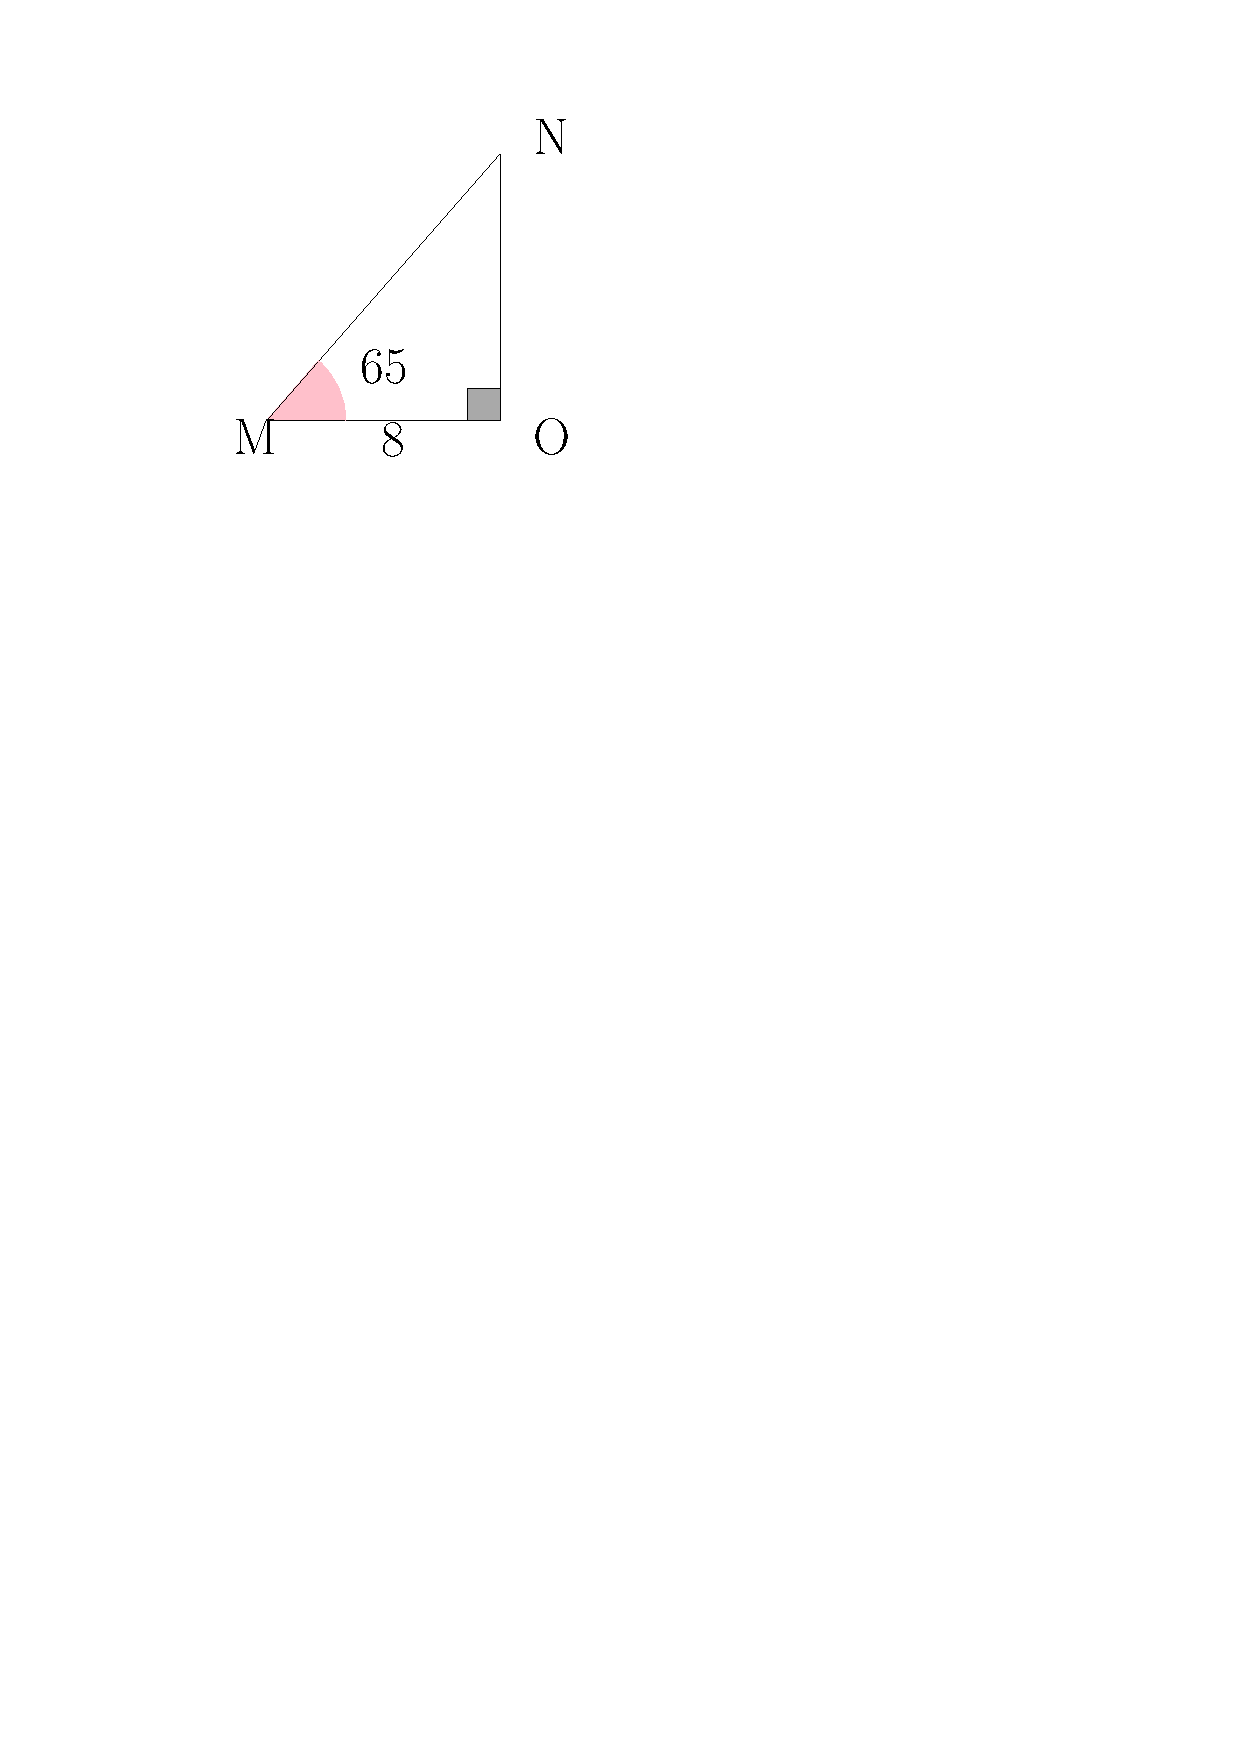
\includegraphics[width=0.6\linewidth]{sources/2/rec-a2.pdf}
	\end{figure}

  \subsubsection*{c) Recherche de $\overbrace{ACB}$}
  
  \begin{figure}[H]
	  \centering
	  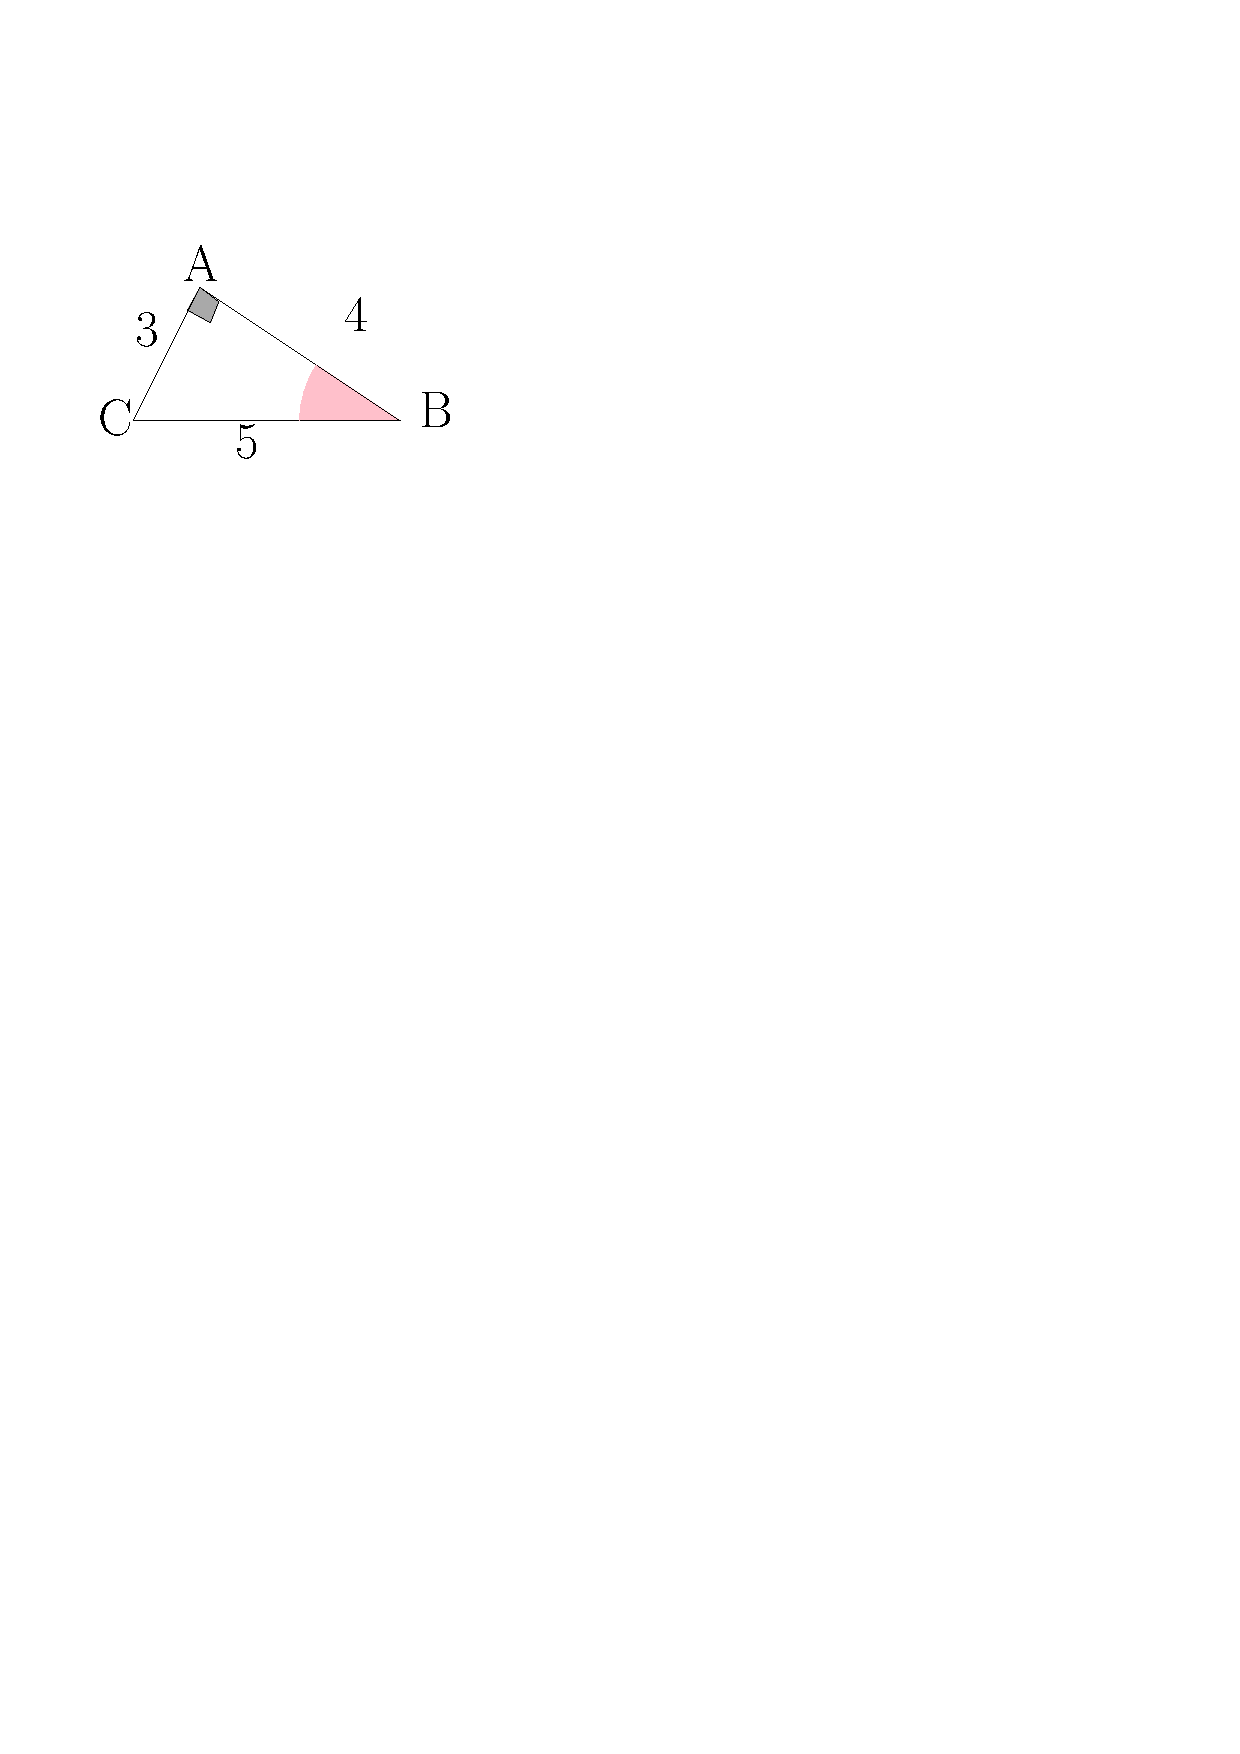
\includegraphics[width=.8\linewidth]{sources/2/rec-a3.pdf}
	\end{figure}
  \end{multicols}

\begin{multicols}{3}

  ABC, un triangle rectangle en C.

  \begin{eqnarray*}
    \cos(\overbrace{CAB}) &=& \dfrac{AC}{AB}             \\
    \cos(42)              &=& \dfrac{AC}{7}              \\
    AC                    &=& 7 \times \cos(42)          \\
    AC                    & \approx & 5.2
  \end{eqnarray*}
  
  \vspace{1cm}
  
  MNO, un triangle rectangle en O.

    \begin{eqnarray*}
      \cos(\overbrace{OMN}) &=& \dfrac{MO}{MN}           \\  
      \cos(65)              &=& \dfrac{8}{MN}            \\
      MN \times \cos(65)    &=& 8                        \\
      MN                    &=& \dfrac{8}{\cos{65}}      \\
      MN                    & \approx & 18.9
    \end{eqnarray*}

  ABC, un triangle rectangle en A.

  \begin{eqnarray*}
    \cos(\overbrace{ACB}) &=& \dfrac{CA}{CB}                       \\
    \cos(\overbrace{ACB}) &=& \dfrac{3}{5}                         \\
    \overbrace{ACB}       &=& \cos^{-1} \left( \dfrac{3}{5} \right) \\
    \overbrace{ACB}       &\approx& 53.1
  \end{eqnarray*}
  
  \end{multicols}   
  
    \paragraph{Remarques}~~\\
  \begin{itemize}
  \item Il faut que la calculatrice soit en \textbf{degré} (et non en radian).
  \item Il faut faire attention aux \textbf{parenthèses}.
  \end{itemize}


\end{document}
